\documentclass[twoside]{report}

% ------
% Umlaute
\usepackage{ifluatex,ifxetex}
\ifluatex
  \usepackage{fontspec}
\else
  \ifxetex
    \usepackage{fontspec}
  \else
    \usepackage{selinput}
    \SelectInputMappings{
      adieresis={ä},
      germandbls={ß},
    }
    \usepackage[T1]{fontenc}
    %\usepackage{textcomp}% optional
    %\usepackage{lmodern}
  \fi
\fi

% ------
% Paper auf Deutsch
\usepackage[ngerman]{babel}

% ------
% Page layout
\usepackage[hmarginratio=1:1,top=32mm,columnsep=20pt]{geometry}
\usepackage[font=it]{caption}
\usepackage{paralist}
%\usepackage{multicol}


% ------
% Abstract
\usepackage{abstract}
	\renewcommand{\abstractnamefont}{\normalfont\bfseries}
	\renewcommand{\abstracttextfont}{\normalfont\small\itshape}


% ------
% Titling (section/subsection)
\usepackage{titlesec}
\renewcommand\thesection{\Roman{section}}
\titleformat{\section}[block]{\Large\scshape\bfseries}{\thesection.}{1em}{}
\setcounter{secnumdepth}{3}

% ------
% Tabellen über Seitenumbrüche hinweg
\usepackage{longtable}

%
% Erweiterte Tabellen
\usepackage{tabularx}
\usepackage{multirow}
\usepackage{float}

%Unterschiedliche Zielgruppen des Dokuments
\usepackage{multiaudience}
\SetNewAudience{developer}
\SetNewAudience{manualDE}


% ------
% Header/footer
\usepackage{fancyhdr}
	\pagestyle{fancy}
	\fancyhead{}
	\fancyfoot{}
\begin{shownto}{-, developer, manualDE}
	\fancyhead[C]{Projektdokumentation $\bullet$ PUML $\bullet$ WS18/19$+$SS19}
	\fancyfoot[RO,LE]{}
\end{shownto}
\begin{shownto}{developer}
	\fancyhead[C]{Entwicklerdokumentation $\bullet$ PUML}
	\fancyfoot[RO,LE]{}
\end{shownto}
\begin{shownto}{manualDE}
	\fancyhead[C]{Benutzerhandbuch $\bullet$ PUML}
	\fancyfoot[RO,LE]{}
\end{shownto}


% ------
% Clickable URLs (optional)
%\usepackage{hyperref}
\usepackage[colorlinks=true,linkcolor=black]{hyperref} %Verlinkung des Inhaltsverzeichnisses ohne roten Rahmen um den Text

% ------
% Literaturverweise mit Bibtex einbinden
\usepackage[authoryear,sectionbib,round]{natbib}

% ------
% Bilder laden
\usepackage[pdftex]{graphicx}

\begin{shownto}{-, developer, manualDE}
% ------
% Maketitle metadata
\title{\vspace{-5mm}%
	\fontsize{24pt}{10pt}\selectfont
	\textbf{Projektdokumentation}
	}	
\author{%
        % alle Autoren hier listen
        % 
	\large
	\textsc{Softwarearchitekt: Philipp Rimmele -- philipp.rimmele@stud.htwk-leipzig.de} \\[2mm]
	\textsc{Product Owner: Anna Heinrich -- anna.heinrich@stud.htwk-leipzig.de} \\[2mm]
	\textsc{Marian Geißler -- marian.geissler@stud.htwk-leipzig.de} \\[2mm]
	\textsc{Patrick Otte -- patrick.otte@stud.htwk-leipzig.de} \\[2mm]
	\textsc{Johann Gerhardt -- johann.gerhardt@stud.htwk-leipzig.de} \\[2mm]
	\textsc{Michael Lux -- michael.lux@stud.htwk-leipzig.de}	\\[2mm]	
	\textsc{Jan Sollmann -- jan.sollmann@stud.htwk-leipzig.de} \\[2mm]
	\textsc{Julian Uebe -- julian.uebe@stud.htwk-leipzig.de} \\[2mm]
	\textsc{Elisabeth Schuster -- elisabeth.schuster@stud.htwk-leipzig.de} \\[2mm]		
	\textsc{Leo Rauschke}	\\[2mm]
	\normalsize	HTWK Leipzig 
	}
\date{}
\end{shownto}
\begin{shownto}{developer}
\title{\vspace{-5mm}%
	\fontsize{24pt}{10pt}\selectfont
	\textbf{Entwicklerdokumentation}
	}	
\author{%
        % alle Autoren hier listen
        % 
	\large
	\textsc{PUML} \\[2mm]
	}
\date{}
\end{shownto}
\begin{shownto}{manualDE}
\title{\vspace{-5mm}%
	\fontsize{24pt}{10pt}\selectfont
	\textbf{Benutzerhandbuch}
	}	
\author{%
        % alle Autoren hier listen
        % 
	\large
	\textsc{PUML} \\[2mm]
	}
\date{}
\end{shownto}


% Erweiterte Tabellen
\usepackage{tabularx}
\usepackage{multirow}
\usepackage{float}

%Tabellen mit Items
\usepackage{booktabs}% http://ctan.org/pkg/booktabs
\newcommand{\tabitem}{~~\llap{\textbullet}~~}

% Code Beispiel Java
\usepackage{listings}
\lstset{
	language=Java,
	aboveskip=2mm,
	belowskip=2mm,
	showstringspaces=false,
	columns=flexible,
	basicstyle={\small\ttfamily},
	numbers=none,
	breaklines=true,
	breakatwhitespace=true,
	tabsize=3
}

% Geschachtelte Sections
\newcounter{sectionlevel}

\newcommand{\nsecbegin}[1]
{
    \ifnum\value{sectionlevel} = 0
    \PackageError{nsection}{Die minimale verschachtelungstiefe wurde unterschritten}
    %\part{#1}%
    \else
    \ifcase\value{sectionlevel} 
    \chapter{#1}
    \or
    \section{#1}
    \or
    \subsection{#1}
    \or
    \subsubsection{#1}
    \or
    \paragraph{#1}
    \or
    \subparagraph{#1}
    \else
    \PackageError{nsection}{Die maximale verschachtelungstiefe wurde ueberschritten}
    \fi
    \fi
    \addtocounter{sectionlevel}{1}
}

\newcommand{\nsecend}
{
  \addtocounter{sectionlevel}{-1}
}

\setcounter{sectionlevel}{1}




%%%%%%%%%%%%%%%%%%%%%%%%
\begin{document}


% -------
% Titel und Abstract über beide Spalten
%\twocolumn[
%\begin{@twocolumnfalse}

\maketitle
\thispagestyle{fancy}

\tableofcontents

%%%%
%%%% Die Struktur des Dokuments bitte nicht aendern!!!
%%%%

\begin{shownto}{-, developer, manualDE}

\nsecbegin{Anforderungsspezifikation}

\nsecbegin{Initiale Kundenvorgaben}
Maecenas sed ultricies felis. Sed imperdiet dictum arcu a egestas. 
In sapien ante, ultricies quis pellentesque ut, fringilla id sem. Proin justo libero, dapibus consequat auctor at, euismod et erat. Sed ut ipsum erat, iaculis vehicula lorem. Cras non dolor id libero blandit ornare. Pellentesque luctus fermentum eros ut posuere. Suspendisse rutrum suscipit massa sit amet molestie. Donec suscipit lacinia diam, eu posuere libero rutrum sed. Nam blandit lorem sit amet dolor vestibulum in lacinia purus varius. Ut tortor massa, rhoncus ut auctor eget, vestibulum ut justo.
\nsecend

% Hier eure Recherchen für den Produktvisions-Workshop ergänzen! Kopiert den Inhalt eures Dokuments einfach in die bereits dafür angelegte Datei. Ihr könnt auch gern selbst eine erstellen, denkt nur daran, die Aufgabenstellung aus Jira zu kopieren, damit am Ende alles schön einheitlich ist.

\nsecbegin{Produktvision}
Es ist ein Entwicklungswerkzeug gewünscht, welches es ermöglicht, für den Quellcode eines bestehenden Softwareprojekts beliebig viele Klassen- und Sequenzdiagramme mittels PlantUML zu erstellen und zu verwalten. Das Werkzeug soll plattformunabhängig und nach Möglichkeit als Plugin in Eclipse integrierbar sein. Das Programm soll sowohl über eine grafische Oberfläche als auch über die Konsole bedienbar sein. Angestrebt ist außerdem die Unterstützung von mehreren Programmiersprachen, wobei das Hinzufügen von neuen Programmiersprachen möglichst einfach ausfallen soll. 
\nsecend

% Das hier ist ein Absatz, der die Grafik in Abbildung~\ref{fig:bild1} detailliert erläutert, erklärt und interpretiert.

% \begin{figure}[b]
%   \centering
%   \includegraphics[width=4.5cm]{bspbild1.png}
%   \caption{Beispiel für ein einspaltiges Bild}
%   \label{fig:bild1}
% \end{figure}


\nsecbegin{Liste der funktionalen Anforderungen}
\nsecbegin{Userstories}
\nsecbegin{Vorschau}
Als Benutzer wünsche ich mir eine Vorschau der Diagramme, damit ich einschätzen kann ob ich damit zufrieden bin.
\nsecend

\nsecbegin{Interfaces}
Als Benutzer wünsche ich mir, dass ich abhängig von Interfaces die zugehörigen Klassen anzeigen lassen kann, damit ich weiß, welche Methoden ich implementieren muss.
\nsecend

\nsecbegin{Kommandozeile}
Als Benutzer wünsche ich mir, dass das Programm von der Kommandozeile aus aufrufbar ist, um es automatisiert starten zu können.
\nsecend

\nsecbegin{Dateien einlesen}
\nsecbegin{Art der eingelesenen Datei}
Als Benutzer wünsche ich mir, dass eine Auswahl zwischen Jar- und Java-Dateien möglich ist, damit Quellcode nicht doppelt eingelesen wird.
\nsecend

\nsecbegin{Java-Dateien}
Als Benutzer wünsche ich mir, dass Java-Dateien einlesbar sind, um den Quellcode von einer oder mehreren Klassen zu analysieren.
\nsecend

\nsecbegin{Jar-Dateien}
Als Benutzer wünsche ich mir, dass Jar-Dateien einlesbar sind, um den Quellcode zu analysieren.
\nsecend
\nsecend

\nsecbegin{Klassendiagramme}
Als Benutzer wünsche ich mir, Klassendiagramme aus meinem bestehenden Quellcode erstellen zu können, damit ich das nicht manuell tun muss.
\nsecend

\nsecbegin{Sequenzdiagramme}
Als Benutzer wünsche ich mir, Sequenzdiagramme aus meinem bestehenden Quellcode erstellen zu können, damit ich das nicht manuell tun muss.
\nsecend

\nsecbegin{Klassenauswahl}
Als Benutzer wünsche ich mir die Möglichkeit, Klassen zu selektieren, damit die Diagramme nicht zu unübersichtlich werden.
\nsecend

\nsecbegin{Methoden- und Variablenauswahl}
Als Benutzer wünsche ich mir die Möglichkeit, Methoden und Variablen zu selektieren, damit die Diagramme nicht zu unübersichtlich werden.
\nsecend

\nsecbegin{Multiple Klassenauswahl}
Als Benutzer wünsche ich mir einen Button, mit dem ich alle Klassen an- oder abwählen kann, damit ich nicht alle Klassen einzeln auswählen muss.
\nsecend

\nsecbegin{Multiple Methodenauswahl}
Als Benutzer wünsche ich mir einen Button, mit dem ich alle Methoden an- oder abwählen kann, damit ich nicht alle Methoden einzeln auswählen muss.
\nsecend

\nsecbegin{Layout}
Als Benutzer wünsche ich mir, das Layout meiner Diagramme ändern zu können, um deren Aussehen zu verbessern.
\nsecend


\nsecbegin{Drag-and-Drop}
Als Benutzer wünsche ich mir, die ausgewählten Dateien oder Ordner per Drag-and-Drop in das Programm aufzunehmen, damit ich den Datei-öffnen-Dialog nicht nutzen muss.
\nsecend

\nsecbegin{Anzeigen und Speichern von PlantUML}
Als Benutzer wünsche ich mir, Diagramme als PlantUML-Code anzeigen und speichern zu können, um den Aufbau nachvollziehen zu können.
\nsecend

\nsecbegin{Speichern von Bilddateien}
Als Benutzer wünsche ich mir, die erstellten Diagramme als Bilddatei exportieren zu können, um sie in meine Projektdokumentation mit aufzunehmen.
\nsecend

\nsecbegin{Speichern von Konfigurationen}
Als Benutzer wünsche ich mir, meine Konfiguration speichern zu können, damit ich meine Präferenz nicht jedes Mal aufs Neue einstellen muss.
\nsecend

\nsecbegin{Benutzerhandbuch}
Als Benutzer wünsche ich mir, das Benutzerhandbuch über die GUI anzeigen lassen zu können, damit ich die gedruckte Version nicht benötige.
\nsecend

\nsecbegin{Übersicht aller Diagramme für ein Projekt}
Als Benutzer wünsche ich mir eine Übersicht aller Diagramme, die ich für mein Projekt erstellt habe, damit ich leichter auf diese zugreifen kann.
\nsecend

\nsecbegin{Drucken}
Als Benutzer wünsche ich mir, Diagramme über das GUI drucken zu können, damit ich die Bilddateien nicht separat öffnen muss.
\nsecend

\nsecbegin{Exceptions als Sequenzdiagramme}
Als Benutzer wünsche ich mir, dass der mögliche Pfad der Exceptions als Sequenzdiagramm angezeigt werden kann, um ungehandelte Exceptions zu vermeiden.
\nsecend

\nsecend
\nsecend

%
% soll der Inhalt dieser Subsection in einer separaten Datei
% (z.B. listefunktional.tex) liegen, dann kann dies mit dem
% folgenden Kommando geschehen.
%
% \input{listefunktional}

\nsecbegin{Liste der nicht-funktionalen Anforderungen}
XXX
\nsecend

\nsecbegin{Weitere Zuarbeiten zum Produktvisions-Workshop}
XXX
\nsecend

\nsecbegin{Zuarbeit der Teammitglieder}
\nsecbegin{Kernfunktionalität}
Denkanstöße:
\begin{itemize}
\item Was soll das Programm auf jeden Fall leisten?
\item Was sind bezogen auf die Funktionalität die Prioritäten im ersten Sprint?
\end{itemize}
Die Kernfunktionalität lässt sich weitgehend aus der Projektbeschreibung ableiten. Ergänzend dazu sollte überlegt werden, ob sich aus dieser Beschreibung noch ungeklärte Fragen ergeben. Die Recherche dient also der Formulierung eines klaren Anforderungsprofils für unser Produkt.
\nsecend
%Autor: Jan Sollmann
\nsecbegin{Anwenderprofil}
Denkanstöße:
\begin{itemize}
\item Wer ist unsere Zielgruppe?


Die Zielgruppe des Projekts beinhaltet alle auf Java programmierenden Personen welche zudem mit UML-Diagrammen meist vorwiegend komplexere Softwareprojekte visualisieren wollen. Spezifischer ist das Programm jedoch an fortgeschrittene bis professionelle Programmierer gerichtet um Softwareprojekte möglichst einfach und nach Wünschen des Nutzers in PlantUML zu überführen.  


\item Worauf legt unsere Zielgruppe besonderen Wert?


Die Zielgruppe fordert einerseits eine einfache Schnittstelle zwischen Quellcode und PlantUML um leicht und bedienerfreundlich automatisch UML-Diagramme zu erzeugen und gegebenenfalls Veränderung an der automatisch erzeugten Visualisierungen vorzunehmen.


\item Was für einen Mehrwert bietet unser Produkt der Zielgruppe?


Der Mehrwert des Projekts liegt bei der Füllung der Lücke zwischen PlantUML und Java-Quelltext, sodass einzelne oder eine Menge von Jar-Dateien automatisch eingelesen werden und in Voransicht dargestellt so bearbeitet werden können, dass der Nutzer die Entscheidungskraft darüber hat, welche Bestandteile in ein Klassen-Diagramm mit eingehen sollen. Zudem hat der Nutzer die Möglichkeit Sequenzdiagramme aus einer oder mehrerer Methoden zu erzeugen. Auch hier wird dem Nutzer eine Einscheidungsgewalt gewährt, bei dieser er bestimmte Aufrufe blockieren und sich bei alternativen Pfaden für einen der selbigen Entscheiden kann. Somit wird eine Diagramm mit Klassen, Verknüpfungen und und use-Beziehungen nach Vorstellungen des Nutzers erstellt.
\end{itemize}
Hier geht es einerseits um eine klare, wenn auch triviale Einordnung, wer unser Produkt später nutzen soll. Andererseits soll erörtert werden, wie das Produkt unserer Zielgruppe das Leben leichter machen kann.
\nsecend

    
    
    



\nsecbegin{PlantUML-Vorstellung (Autor: Marian Geißler)}

Diese Recherche soll einen kurzen, ersten Einblick in den Aufbau und die Möglichkeiten von PlantUML gewähren.\\
Beschreibung in PlantUML
\begin{itemize}
\item web server unter: http://www.plantuml.com/plantuml/ für kleine Test, zum ausprobieren

\item Syntax\\
Beginn mit: „@startuml“
Ende:  „@enduml“\\
Kein „;“ zur Abgrenzung\\
Neue Zeile für neue Anweisung\\
Bsp.:\\
\begin{lstlisting}
@startuml
Bob -> Alice
@enduml
\end{lstlisting}

\item Klassen\\
- Werden durch Schlüsselwort „class“ eingeleitet\\
- Kann Attribute und/oder Methoden erhalten\\
- Bei längeren Klassen „…lange Klasse…“ as long\\
- Sichtbarkeit der Klasse über Symbole Minus, Tilde, Plus und Doppelkreuz\\
- Attribute und Merkmale können „Abstract“ oder „Static“-Merkmale bekommen über geschweifte Klammern\\
\\
Bsp. 1 - Einzelne Klasse:\\
\begin{lstlisting}
@startuml
class ErsteKlasse
@enduml
\end{lstlisting}
Bsp. 2 - Klasse mit langem Namen:\\
\begin{lstlisting}
@startuml
class "wirklich alleralleraller ErsteKlasse" as long
@enduml
\end{lstlisting}
Bsp. 3 - Klasse mit Methode und Datendeklaration:\\
\begin{lstlisting}
@startuml
class ErsteKlasse : Name
@enduml
Bsp.:
@startuml
class ZweiteKlasse{
String name
Integer wert
void methode(String parameter1, Int parameter2)
}
@enduml
\end{lstlisting}
Bsp. 4 - Sichtbarkeit der Klassen:\\
\begin{lstlisting}
Bsp.:
@startuml
class MeineKlasse{
- Private
# Protected
~ PackagePrivate
+ Public
}
@enduml
\end{lstlisting}
Bsp. 5 -  Static / Abstract:\\
\begin{lstlisting}
@startuml
class MeineKlasse{
      {static} String password
      {abstract} void methods()
      }
@enduml
\end{lstlisting}
Bsp. 6 - Abstrakte Klasse\\
\begin{lstlisting}
@startuml
abstract class AbstrakteZweiteKlasse
@enduml
\end{lstlisting}
Bsp. 7 . Interface\\
\begin{lstlisting}
@startuml
interface schoenesInterface
@enduml
\end{lstlisting}
\item Klassen Verbinden\\
- einfach\\
- gerichtet in eine Richtung\\
- in Beide Richtungen gerichtet\\
Bsp. 1 - Einfache Verbindung\\
\begin{lstlisting}
@startuml
class ErsteKlasse
class ZweiteKlasse
ErsteKlasse -- ZweiteKlasse
\end{lstlisting}
Bsp. 2 - Gerichtete Verbindung\\
\begin{lstlisting}
@startuml
class ErsteKlasse
class ZweiteKlasse
ErsteKlasse --> ZweiteKlasse
@enduml
\end{lstlisting}
Bsp. 3 - In beide Richtungen gerichtet\\
\begin{lstlisting}
@startuml
class ErsteKlasse
class ZweiteKlasse
ErsteKlasse <--> ZweiteKlasse
@enduml
\end{lstlisting}
Bsp. 4 - Lose-Verbindung\\
\begin{lstlisting}
@startuml
class ErsteKlasse
class ZweiteKlasse
ErsteKlasse o-- ZweiteKlasse
@enduml
\end{lstlisting}
Bsp. 5 - Gebundene Klassen\\
\begin{lstlisting}
@startuml
class ErsteKlasse
class ZweiteKlasse
ErsteKlasse *-- ZweiteKlasse
@enduml
\end{lstlisting}
Bsp. 6 - Vererbung Unterlass/Oberklasse\\
\begin{lstlisting}
@startuml
class ErsteKlasse
class ZweiteKlasse
ErsteKlasse o--|> ZweiteKlasse
@enduml
\end{lstlisting}
Bsp. 7 - Notiz\\
\begin{lstlisting}
@startuml
class ErsteKlasse
class ZweiteKlasse
ErsteKlasse -- ZweiteKlasse
note ``Dies ist`` as notiz1
ErsteKlasse .. notiz1
\end{lstlisting}
\item Pfeile
- kurze Pfeile/ lange Pfeile (-/—) unterschied Anordnung\\
- für includes und extends (..)\\
Bsp. 1 - kurz\\
\begin{lstlisting}
@startuml
class ErsteKlasse
class ZweiteKlasse
ErsteKlasse -> ZweiteKlasse
@enduml
\end{lstlisting}
Bsp. 2 - lang\\
\begin{lstlisting}
@startuml
class ErsteKlasse
class ZweiteKlasse
ErsteKlasse --> ZweiteKlasse
@enduml
\end{lstlisting}
Bsp. 3 - gestrichelt\\
\begin{lstlisting}
@startuml
class ErsteKlasse
class ZweiteKlasse
ErsteKlasse..> ZweiteKlasse
@enduml
\end{lstlisting}
Bsp. 4 - include und extend Assoziation\\
\begin{lstlisting}
Bsp2. gestrichelt - include und extend Assoziation:
@startuml
(A) .> (B): <<include>>
(B) .> (C): <<extend>>
@enduml
\end{lstlisting}
Bsp. 5 - Weitere Kombinationen zum Test auf www.plantuml.com/plantuml/\\
\begin{lstlisting}
@startuml
Bob -> Alice: synchrone Nachricht von Bob an Alice
Bob ->> Alice: asynchrone Nachricht von Bob an Alice
Bob --> Alice: gestrichelte Linie als Antwortnachricht
Bob -\ Alice: Pfeilspitze ist nur oberhalb der Linie gezeichnet
Bob ->x Alice: verlorene Nachricht von Bob an Alice, x an Pfeilspitze
Bob \\- Alice: Pfeilspitze ist nur unterhalb angezeigt, jedoch offen
Bob //-- Alice: gestrichelte Linie mit offener Pfeilspitze oberhalb
Bob ->o Alice: Kreis am Ende der Pfeilspitze auf der Lebenslinie von Alice Bob <-> Alice: bidirektionaler Pfeil
Bob <->o Alice: bidirektionaler Pfeil mit Kreis am Ende der Pfeilspitze
@enduml
\end{lstlisting}
\item Beschriftungen der Verbindungen\\
- einfache Annotationen durch „:“\\
- mit Richtungsangabe\\
Bsp. 1 - Simple Beschriftung\\
\begin{lstlisting}
@startuml
class ErsteKlasse
class ZweiteKlasse
ErsteKlasse - ZweiteKlasse : Beschriftung mit Leerzeichen
@enduml
\end{lstlisting}
Bsp. 2 - Beschriftung mit Leserichtung\\
\begin{lstlisting}
@startuml
class ErsteKlasse
class ZweiteKlasse
ErsteKlasse - ZweiteKlasse : Beschriftung mit Leserichtung <
@enduml
\end{lstlisting}
\item Limitierung der Darstellung in PlantUML\\
-keine direkten Verzweigungen, immer an Element gekoppelt\\
- es können inkonsistente Zeichnungen entstehen\\
Bsp. 1 - Vererbung im Kreis:
\begin{lstlisting}
@startuml
class a
class b
a -|> b
b -|> a
note "Fehler" as notiz1 a .. notiz1
@enduml
\end{lstlisting}
\item UML Erweiterungen von Interesse\\
Unterstützung für: \\
- Java API (plantuml.jar)\\
- png from String -png from File -svg from String\\
- Command Line/Terminal\\
- Eclipse (Plug-In)\\
- LaTex\\
- Atom, GEdit, VIM, weitere txt-editoren...\\
\end{itemize}

\nsecend

\nsecbegin{Konkurrenzprodukte (Autor: Julian Uebe)}
%Denkanstöße:
%\begin{itemize}
%\item Gibt es schon ähnliche Ansätze?
%\item Wie unterscheiden / gleichen sich diese bezogen auf ihre Funktionalität?
%\item Welche Nischen gibt es?
%\end{itemize}
%Hier sollen sowohl Marktlücken als auch "Best Practices" identifiziert werden.
\begin{itemize}
	\item ähnliche Ansätze:
	\begin{itemize}
		\item bisher nur z.B. Umwandlung von PlantUML-Code zu Quelltext oder XMI-Dateien
		\item Eclipse-Plugin zum Anzeigen von PlantUML-Code aber nicht zum Generieren
	\end{itemize}
	\item Object-Aid:
		\begin{itemize}
			\item Plugin für Eclipse zum Generieren von UML-Diagrammen aus Quelltext
			\item keine Unterstützung von PlantUML
			\item Drag \& Drop möglich
			\item nicht Open Source
			\item Klassendiagramme sind frei zugänglich
			\item Sequenzdiagramme benötigen kostenpflichtige Lizenz
		\end{itemize}
	\item hpp2plantUML:
		\begin{itemize}
			\item quelloffener Konverter von C++-Qellcode zu PlantUML-Code
		\end{itemize}
\end{itemize}
Fazit:
Es gibt einige Ansätze, die bereits teilweise unsere geplanten Funktionalitäten implementieren.
Letztendlich lässt sich aber sagen, dass es noch kein Projekt gibt, was im vollen Umfang unsere Aufgaben abdeckt.
\nsecend
\nsecbegin{Mögliche Weiterentwicklung}
Denkanstöße:
\begin{itemize}
%\item Wie können wir unser Produkt verbessern, sobald es die definierten Kernfunktionalitäten enthält?
%\item (Am besten mit der Person erörtern, die zu Konkurrenzprodukten recherchiert) Welche Features bietet die Konkurrenz, die wir nicht für die Kernfunktionalität festgelegt haben?
%\item Grob geschätzt: Wie nützlich sind diese Features und wie aufwendig wäre deren Implementierung?
	\item Einlesen von Projekten aus verschiedenen Programmiersprachen
	\begin{itemize}
		\item Beispielsweise:
		\begin{itemize}
			\item Python
			\item C++
			\item C\#
			\item etc.
		\end{itemize}
			\item Nützlichkeit:
		\begin{itemize}
			\item Erhöht Einsetzbarkeit des Tools enorm
			\item Erhöht die Anzahl der möglichen Nutzer des Tools
		\end{itemize}
			\item Umsetzbarkeit:
		\begin{itemize}
			\item Durch die XML-Schnittstelle muss alleinig der Parser angepasst werden
			\item Den Parser ist allerdings die aufwendigste Klasse des Programms
		\end{itemize}
	\end{itemize}
	\item Erstellung eines Eclipse Plugins
	\begin{itemize}
		\item Nützlichkeit:
		\begin{itemize}
			\item Erhöht Usebility enorm
			\item Erleichtert die Benutzung
			\item Vergrößert die wahrscheinliche Anzahl der Nutzer durch einfache Einbindung
		\end{itemize}
			\item Umsetzbarkeit:
		\begin{itemize}
			\item Umsetzung durch Umsetzung in Konkurenzprodukten erleichtert
			\item Wahrscheinlich in geplantem Zeitraum umsetzbar
		\end{itemize}
	\end{itemize}
	\item Anpassen des Quellcodes durch Änderungen im erstellten UML Diagramm
	\begin{itemize}
		\item Nützlichkeit:
		\begin{itemize}
			\item Erhöht die Nutzbarkeit des Tools als ein Gesamtprodukt durch komplette Funktionalität
			\item Gibt dem Tool eine flexiblere Nutzbarkeit
		\end{itemize}
			\item Umsetzbarkeit:
		\begin{itemize}
			\item In vorgegebener Zeit schwer realisierbar
			\item Mögliche Erweiterung als weiterführendes Projekt
		\end{itemize}
	\end{itemize}
	
\end{itemize} %endTag
%Hier wurde z.B. schon eine Implementierung als Eclipse-Plugin und Support für verschiedene Programmiersprachen angesprochen.
\nsecend
\nsecbegin{GUI-Anforderungen (Autor: Michael Lux)}
Denkanstöße:
\begin{itemize}
\item Wie könnte das User Interface aussehen?

\item Wie können wir für eine gute User Experience sorgen?
\end{itemize}
Auch, wenn die GUI im ersten Sprint nur in Grundzügen entwickelt wird, sollten wir uns früh Gedanken über deren Aussehen und Funktionalität machen. Dazu gehört, wie der Workflow abläuft und wie wir das GUI unserer Anwendung darauf zuschneiden können. Welche großen roten Knöpfe brauchen wir, welche Funktionen dürfen in dreifach verschachtelten Untermenüs versteckt werden?

Eine Möglichkeit fur das Aussehen und Funktionalität wäre folgende:

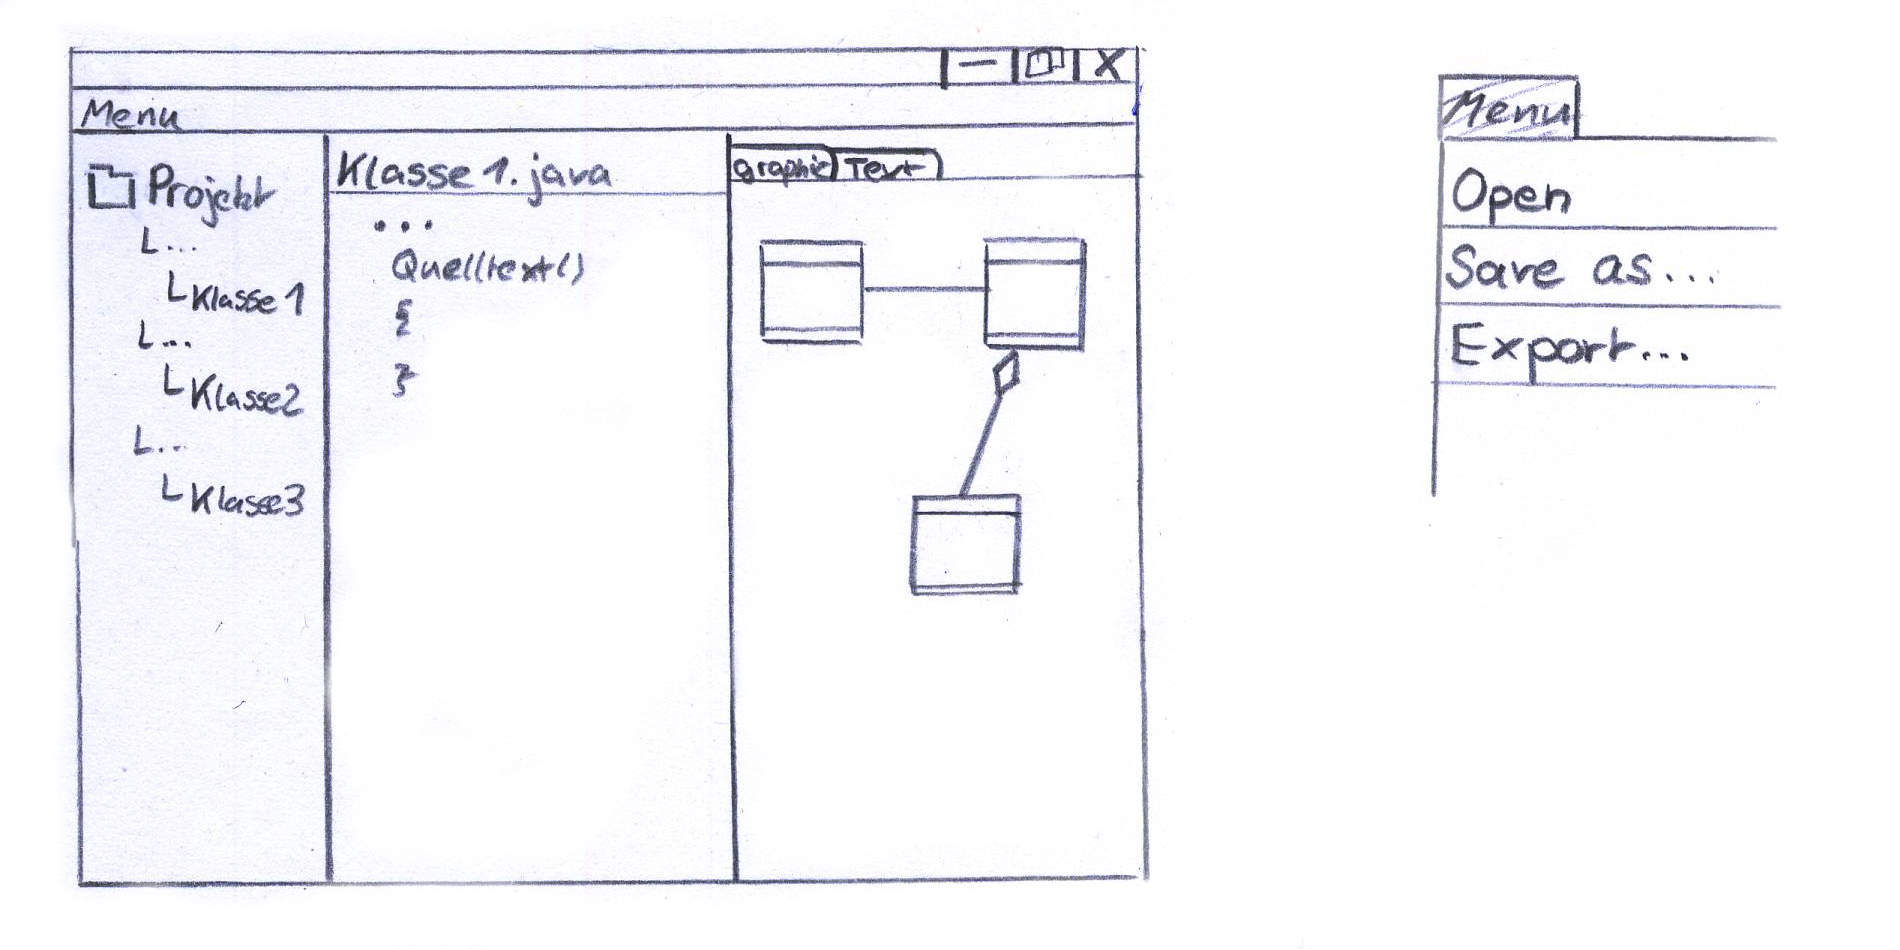
\includegraphics[]{Bilder/GUI-Beispiel.png}

Die wichtigsten Funktionalitäten verbergen sich im Untermenü unter Menü.
Ein Projekt bzw. eine Datei mit verschiedenen Klassen soll dort unter „Open“ geöffnet werden.
Das Programm erzeugt daraus automatisch die UML, die rechts entweder grafisch, oder in Textform dargestellt wird. (Auswahl durch Tabs)
Links ist die Klassenhierarchie und der Quelltext der jeweiligen Klasse bzw. Datei zu sehen.
Die erstellte UML soll durch den Benutzer per Maus- und Tastatureingaben in der UML selbst verändert werden können. (Beispiel: Verschieben einer Klasse mit der Maus)
Anschließend soll der Anwender die Möglichkeit haben, die UML grafisch als Bilddatei oder in Textform speichern zu können über die Funktionen „Save as“ und „Export“.
\nsecend
\nsecbegin{Datenmodell (Autor: Elisabeth Schuster)}
\begin{itemize}
\item Welche Daten verarbeiten wir?
\begin{itemize}
\item Quellcode, der vom Anwender gegeben wird
\item Daten sind abhängig vom Nutzer
\end{itemize}
\item Form der Datenaus- und -eingabe
\begin{itemize}
\item Eingabe: Jar-Datei oder mehrere Java-Dateien, die Quellcode enthalten oder Textdateien
\item Ausgabe: Klassendiagramme, Sequenzdiagramme, ... mit den Beziehungen zwischen den einzelnen Klassen
\end{itemize}
\item wichtige Variablen und Parameter
\begin{itemize}
\item Klassenname
\item Klassenattribute
\item Relationen zwischen den einzelnen Klassen (mit Pfeilen dargestellt)
\item Methoden der einzelnen Klassen
\item Eigenschaften wie abstract, private, protected, etc.
\end{itemize}
\item wichtige Klassen aus der Java-Standardbibliothek
\begin{itemize}
\item java.awt - zum Erstellen von User-Interfaces
\item jav.io - zum Einlesen von Dateien
\item java.util - enthält z.B. event model, frameworks, internationalization, ...
\item javax.swing - enthält Klassen zum Erstellen einer GUI
\end{itemize}
\end{itemize}
\nsecend
\nsecbegin{Erste User-Story}
Denkanstöße:
\begin{itemize}
\item Stell dir vor, das Produkt ist gerade fertig entwickelt worden und deine Teamleiter wollen ein Plant-UML von deinem Quellcode sehen (PUMLception). Welchen Workflow erwartest du? Was machst du in welcher Reihenfolge?
\item Optional: Besprich dich mit dem / der Recherchierenden für die GUI-Anforderungen. Habt ihr unterschiedliche Vorstellungen vom Workflow und wenn ja, wie unterscheiden sie sich?
\item Wie würde für dich rein intuitiv das Graphical User Interface aussehen? Wenn du das GUI mit nur drei Knöpfen bauen müsstest, welche Funktionen würdest du ihnen zuweisen?
\end{itemize}
Workflow:
\begin{enumerate}
\item Wähle im Programm „Öffnen“ aus und suche im Explorer die Datei
\item Datei wird eingelesen und verarbeitet
\item Ich sehe das ganze UML Diagramm auf der einen Seite und den Quelltext auf der anderen
\item Im Quelltext kann ich einzelne Parts auswählen, wodurch kleinere UML Diagramme erstellt werden
\item Ich kann die Anordnung der dargestellten Elemente verändern
\item Nun besteht die Möglichkeit das Diagramm z.B. als png-Datei zu exportieren
\end{enumerate}

GUI:
\begin{itemize}
\item Ganz oben wären Button zum minimieren, maximieren und schließen. Darunter eine Menüleiste mit verschiedenen Optionen um Quelltext und UML-Diagramme zu öffnen und speichern.
\item Am linken Rand ist die Klassenstruktur, wie man sie z.B. in Eclipse hat dargestellt zur Koordination. Direkt daneben befindet sich ein Feld mit dem Quelltext, damit man sich direkt dort vergewissern kann, wie Klassen, die im UML-Diagramm dargestellt sind miteinander im Quelltext interagieren.
\item Auf der linken Seite ist das UML Diagramm dargestellt.
\item Die drei wichtigsten Knöpfe der GUI wären: Öffnen, Speichern und Diagramm bearbeiten
\end{itemize}




\nsecend
\nsecbegin{Workshop-Bedarfsermittlung (Autor: Johann Gerhardt)}
Denkanstöße:
\begin{itemize}
\item Was für Kompetenzen könnten dem Team für die Entwicklung des Produkts fehlen?
\end{itemize}
Um die Recherche hier zu vereinfachen, wäre es nicht schlecht, wenn die anderen Recherchierenden den Bearbeitenden auf mögliche Wissenslücken aufmerksam machen. Ziel dieser Recherche ist ein allgemeiner Überblick, wo Defizite vorhanden sind. Es ist zu vermuten, dass die anfänglich identifizierten Probleme eher abstrakter Natur sind - konkrete "Baustellen" zeigen sich für gewöhnlich erst in der Entwicklung. Erwartet werden also keine haargenauen Angaben zu Kompetenzen bzw. Inkompetenzen.
\\
Fehlende Kompetenzen für die Entwicklung des Produktes:
\begin{itemize}
\item Keine UML-Kenntnisse
\item Keine Programmierkenntnisse welche über die bisherigen Anforderungen des Studiums hinausgehen
\item Keine Erfahrungen mit größeren Gruppenarbeiten
\item Keine bisherige GUI-Programmierung mit Hilfe von Tools
\item Noch nie mit GIT gearbeitet
\item Keine Kenntnisse der Fähigkeiten der Gruppenmitglieder
\end{itemize}

Genannte Stichpunkte treffen zwar meist nicht auf alle, aber dennoch auf einen Großteil der Gruppe zu.
Im Laufe des Projekts werden die meisten fehlenden Kompetenzen automatisch wegfallen, da diese auf Erfahrungen aufbauen. Das Arbeiten mit GIT zum Beispiel wird sicherlich nach mehreren Benutzen einfacher.
\nsecend

\nsecbegin{Workshop-Recherche (Autor: Leo Rauschke)}
Denkanstöße:
\begin{itemize}
\item Wie können wir die Teammitglieder effektiv und effizient auf einen Stand bringen?
\item Welche Ressourcen könnten dafür nützlich sein (Scripting-APIs, gute Tutorials etc.)?
\item Wie können wir die gefundenen Ressourcen so zur Verfügung stellen, dass jeder einfach darauf zugreifen kann?
\end{itemize}
Diese Recherche ist einerseits eng mit der Recherche "Workshop-Bedarfsermittlung" verbunden, es schadet also auf jeden Fall nicht, sich über deren Ergebnisse zu informieren. Aber auch unabhängig davon können schon erste Ideen entwickelt werden, wie das Team miteinander und voneinander lernen kann.

\nsecbegin {Terminabsprache/Mitteilen von Neuigkeiten}
Zur Terminabsprache eignet sich gut ein Messenger wie zB Telegram, wo das Team eine Gruppe hat, übe die Neuigkeiten und Termine schnell ausgetauscht werden können und sich gebündelt an einem Ort befinden. 
\nsecend
\nsecbegin {Gefundene Ressourcen zur Verfügung stellen}
Es wäre sinnvoll, gefundene Ressourcen wie zum Beispiel Dokumente über einsetzbare Technologien, Tutorials oder andere Hintergrundinformationen außerhalb vom Gruppenschat teilen zu können, das können wir über git machen. 
\nsecend


\nsecend



\nsecend

\nsecbegin{Zuarbeit von Autor Y}
XXX
\nsecend

\nsecbegin{Liste der Kundengespräche mit Ergebnissen}
\begin{table}[H]

\begin{tabularx}{\textwidth}{ |l|X|X| }
  \hline
  \textbf{Datum} & \textbf{Anliegen oder Fragen} & \textbf{Ergebnisse}\\
  \hline
  \multirow{2}{*}{02.11.18} & Wie genau soll das Layout des Diagramms anpassbar sein? & Das Layout soll sowohl manuell als auch automatisch optimiert werden können. \\\cline{2-3}
  & Reicht es für den ersten Sprint, wenn PUML als Kommandozeilenprogramm umgesetzt wird? & Es soll möglichst früh eine grafische Oberfläche entwickelt werden. Deren Funktionsumfang darf zu Beginn ruhig minimal sein. Wichtig ist, dass das Team möglichst früh einen \glqq optischen Erfolg\grqq{} zu verzeichnen hat. \\
  \hline
\end{tabularx}
\end{table}

\nsecend

\nsecend %Anforderungsspezifikation

\nsecbegin{Architektur und Entwurf}

\nsecbegin{Zuarbeiten der Teammitglieder}
\nsecbegin{Commandline Funktionalität (Autor: Marian Geißler)}
Eine der Anforderungen an die Software ist die Bedienung des Programms mittels Kommandozeile. Folgende zwei Möglichkeiten scheinen für die Verwendung im Projekt PUML als sinnvoll. Zum einen ist die Parameterabfrage über eine eigene Implementation auf Basis der Hauptklasse möglich mittels \texttt{public static void main(String [] args)}, zum Anderen ist die Nutzung der \glqq Commons CLI\grqq-Bibliothek von Apache eine Option. \\
Während der Recherche zeigte sich, dass die Nutzung der Commons CLI - Bibliothek sehr gut dokumentiert ist und in der Praxis oft Anwendung findet, auch das Umsetzen eines Tests schien weniger problematisch zu gelingen, als ein Abfragen der Parameter über \texttt{String [] args} im Hauptprogramm. Aus diesem Grund wird an dieser Stelle die Apache Bibliothek kurz vorgestellt. \\
Ein Download der Bibliothek erfolgt über die Seite des Enticklers Apache\footnote[1]{http://commons.apache.org/proper/commons-cli/} und muss anschließend in die Entwicklungsumgebung eingebunden, sowie in das Programm importiert werden. \\
Die Arbeit mit Commons CLI lässt sich grundsätzlich in drei Schritte unterteilen, Parameterdefinition, das Einrichten des Parsers und die Verkettung mit der jeweiligen Funktion. \\
Zuerst wird festgelegt, welche Parameter der Anwendung übergeben werden, hierzu wird ein neues Container Objekt vom Typ \texttt{Options} angelegt. Anschließend werden die gewünschten Befehle mit den entsprechenden Parametern dem Container hinzugefügt, so dass später ein Aufruf im Terminal möglich ist, wie bespielsweise \texttt{ls -al meinfile.txt} um die Zugriffsrechte einer Datei zu überprüfen.
\begin{lstlisting}
//Erzeugt neuen Container fuer Programmparameter
Options options = new Options();
//Hinzufuegen einer neuen Option 
options.addOption("l",false, "Alle Leerzeichen entfernen.");
\end{lstlisting}
Zunächst wird ein Parser intitialisert, während anschließend über eine logische Verknüpfung der Flags die entsprechende Funktion aufgerufen wird. Wichtig ist in diesem Zusammenhang noch die Verwendung von Exceptions zu erwähnen, die entweder durch den Ausdruck \texttt{ParseException} aus der Bibliothek oder \texttt{try / catch} Schlüsselwörter abgefangen werden müssen.
\begin{lstlisting}
CommandLineParser parser = new DefaultParser();	
CommandLine commandLine = parser.parse(options,args);

 if(commandLine.hasOption("b"))
{
	System.out.println("String eingebe: ");
	String myString = keyboard.nextLine();	//String einlesen
	getWordBefore('.',myString); // liefere alle Woerter vor Punkt
}
if (commandLine.hasOption("l"))
{
	String myString = "g e s p e r r t g e s c h r i e b e n";
	System.out.println(noSpace(myString));	//entfernt alle Leerzeichen
}
\end{lstlisting}
Am Ende muss das Programm übersetzt werden und steht anschließend zur Nutzung mit den gesetzten Parametern zur Verfügung. So liefert in diesem Fall die Eingabe im Terminal: \texttt{java MeinProgrammName -l } die Ausgabe \glqq gesperrtgeschrieben\grqq zurück.
\nsecend

\nsecbegin{GUI}

\nsecbegin{Welche GUI-Frameworks gibt es für Java?}
Aktuell gibt es folgende Möglichkeiten zur Erstellung einer GUI Oberfläche in Java:
 \begin{itemize}
	\item Swing
	\item JavaFX
	\item Standard Widget Toolkit (SWT)
	\item Abstract Window Toolkit (AWT)
	\item Google Web Toolkit (GWT)
	\item Qt (Qt Jambi)
	\item GTK+
\end{itemize}
\nsecend

\nsecbegin{Welche können für das Projekt genutzt werden?}
Für unser Projekt kommen aktuell die Frameworks Swing und JavaFX in Frage. Zum Einen sind beide aktuell die beiden meist genutzten GUI Frameworks in Java, zum Anderen sind hierfür Eclipse Plugins verfügbar.
\nsecend

\nsecbegin{Vor- und Nachteile der Frameworks}

\textbf{Swing}

\textbf{Vorteile}
\begin{itemize}
	\item Bestandteil des Java Development Kits/Java Foundation Classes
	\item Nutzt eine Sammlung von Bibliotheken zur GUI-Programmierung (Bspw. AWT)
\end{itemize}


\textbf{Nachteile}
\begin{itemize}
	\item Wird nicht mehr weiterentwickelt oder gewartet
	\item Probleme im Bereich Medieneinbindung und Animation
	\item Bestimmte Anwendung wie bspw. Zooming nicht möglich
\end{itemize}



%\begin{info}
	%Swing ist eines der meistgenutzten GUI-Frameworks für Java, war bis 2014 ein Standard-Tool zur GUI Entwicklung und hat aufgrund dessen eine große Community hinter sich und man findet viel Hilfestellungen für Swing im Internet.
%\end{info}
\nsecend

\textbf{JavaFX}

\textbf{Vorteile}
\begin{itemize}
	\item Teil jeder neuen Java SE Installation
	\item Möglichkeit einfach animierte Übergänge einzubinden
	\item optisch ansprechender
	\item Anwendung kann mittels CSS bearbeitet werden (durch Einbindung von FXML-Code)
\end{itemize}


\textbf{Nachteile}
\begin{itemize}
	\item weniger Online-Hilfe, kleinere Community
\end{itemize}


%\begin{info}
	%Aufgrund der erst kurzen Zeit, in der JavaFX zur Verfügung steht, gibt es hier viel weniger Hilfe online im Vergleich zu Swing. JavaFX gilt allerdings als der neue Standard in der Java GUI Entwicklung und es gibt sehr viele Developer, die von Swing zu JavaFX umsteigen.
%\end{info}
\nsecend
\nsecend

\nsecbegin{Fazit}

In Hinsicht auf die Langlebigkeit bzw. der Zukunftssicherheit, der moderneren Optik, der Einbindung in Eclipse und dem steigenden Support haben wir uns für JavaFX zur GUI Entwicklung in unserem Projekt entschieden.

\nsecend
\nsecend
\nsecbegin{Reguläre Ausdrücke (Autor: Elisabeth Schuster)}
Reguläre Ausdrücke sind Beschreibungen eines Musters, sog. Patterns, die bei Zeichenkettenverarbeitung eingesetzt werden. Mittels dieser Muster lassen sich Zeichenketten suchen und ersetzen.\\
\nsecbegin{Funktionen}
\begin{itemize}
\item[(1)] Komplette Übereinstimmung suchen \\
\begin{tabular}{l c}
\begin{lstlisting}
Pattern.matches(regex, this);
\end{lstlisting} & \begin{lstlisting}
Pattern p = Pattern.compile(regex);
Matcher m = p.matcher(input);
return m.matches();
\end{lstlisting} \\
\end{tabular}
\item[(2)] Teilstring finden
\begin{itemize}
\item[$\bullet$] alle Vorkommen des Teilstrings innerhalb eines Suchstrings suchen
\end{itemize}
\item[(3)] Teilfolgen ersetzen
\item[(4)] Zerlegen einer Zeichenfolge
\begin{itemize}
\item[$\bullet$] Trennzeichen sind durch Muster definiert, resultiert in Sammlung von Zeichenfolgen
\end{itemize}
\end{itemize}
\nsecend
\nsecbegin{Verwendung}
\begin{itemize}
\item[]Um mit Regulären Ausdrücken arbeiten zu können, wird das Paket ‚java.util.regex‘ implementiert. Es enthält die Klassen Matcher (Zugriff auf Mustermaschine) und Pattern (Repräsentation RE in vorkompiliertem Format).
Außerdem gibt es verschieden Klassifizierungen, um die Suche genauer zu definieren.
\end{itemize}
%Tabelle1
\begin{table} [H]
\centering
\begin{tabular}{l|c}
\multicolumn{1}{l}{\textbf{Quantifizierung}} & \textbf{Anzahl der Wiederholungen}\\
\hline
X? & X kommt einmal oder keinmal vor \\
\hline
X* & X kommt keinmal oder beliebig oft vor \\
\hline
X+ & X kommt einmal oder beliebig oft vor \\
\hline
X\{n\} & X muss genau n-mal vorkommen \\
\hline
X\{n,\} & X kommt mindestens n-mal vor \\
\hline
X\{n,m\} & X kommt mindestens n-, aber max. m-mal vor \\
\hline
\end{tabular}
\end{table}
%Tabelle2
\begin{table} [H]
\centering
\begin{tabular}{l|c}
\multicolumn{1}{l}{\textbf{zeichenklasse}} & \textbf{Enthält}\\
\hline
. & jedes Zeichen \\
\hline
[aei] & Zeichen a, e, i \\
\hline
[\^{}aei] & nicht die Zeichen a, e, i \\
\hline
[0-9a-f] & Zeichen 0-9 oder Kleinbuchstaben a-f \\
\hline
\textbackslash d & Ziffer: [0-9] \\
\hline
\textbackslash D & keine Ziffer: [\^{}0-9] bzw. [\^{}\textbackslash d] \\
\hline
\textbackslash p\{Blank\} & Leerzeichen oder Tab: [\textbackslash t] \\
\hline
\textbackslash p\{Lower\}, \textbackslash p \{Upper\} & Klein-/Großbuchstaben: [a-z] bzw. [A-Z] \\
\hline
\end{tabular}
\end{table}
weitere Klassifizierungen: \\
\href{https://docs.oracle.com/javase/7/docs/api/java/util/regex/Pattern.html}{https://docs.oracle.com/javase/7/docs/api/java/util/regex/Pattern.html}
\nsecend
\nsecbegin{Beispiele}
\begin{itemize}
\item[(1)] Rückgabewert beider Abfragen ist true
\begin{lstlisting}
System.out.println(Pattern.matches("'.*'","'Hallo Welt'" ));
System.out.println("'Hallo Welt'".matches("'.*'"));
\end{lstlisting}
\item[(2)] Abfrage nach Teilstring, Rückgabewert ist gefundener Teilstring
\begin{lstlisting}
String text = "Moderne Programmiersprachen haben durch die Vernetzung von Computern neue Anforderungen erfahren. So lautet auch ein Motto von Sun: 'The Network is the Computer.' ";
Matcher matcher = Pattern.compile("'.*'").matcher(text);
while(matcher.find()) {
	System.out.println(matcher.group());
}
\end{lstlisting}
\end{itemize}
\nsecend
\nsecend
\nsecend

\nsecbegin{Entscheidungen des Technologieworkshops}
XXX
\nsecend

\nsecbegin{Überblick über Architektur}
XXX
\nsecend

\nsecbegin{Definierte Schnittstellen}
XXX
\nsecend

\nsecbegin{Liste der Architekturentscheidungen}
%XXX (bewusste und unbewusste Entscheidungen mit zeitlicher Einordnung)

\begin{table}[h]
\centering
\begin{tabular}{|l|l|}
\toprule
Zeit & Entscheidung \\
\midrule
Bei Projektvergabe & Als Programmiersprache wird Java verwendet.\\
& Begründung der Entscheidung:\\
&      \tabitem Platformunabhängigkeit\\
&      \tabitem Alle aus dem Team beherschen Java\\
&      \tabitem Sauber und Einsteigerfreundlich\\
&      \tabitem Weiterentwicklung zu Eclipse-Plugin möglich\\
&      \tabitem Ausgereifte GUI-Frameworks verfügbar\\
\midrule
Technologieworkshop & \\
\bottomrule
\end{tabular}
\end{table}
\nsecend


\nsecend %Architektur und Entwurf

\end{shownto} %{-, developer, manualDE}
\begin{shownto}{-, manualDE}

\nsecbegin{Prozess- und Implementationsvorgaben}

\nsecbegin{Definition of Done}
XXX
\nsecend

\nsecbegin{Coding Style}
Bitte die Datei javaCodeStyle.xml im specification-Verzeichniss in Eclipse importieren und verwenden.
Hierfür in Eclipse unter "`Window->Preferences->Java->Code Style->Formatter"' auf Import klicken und die XML-Datei auswählen.\\
Ist der passende Coding Style eingestellt kann der Quellcode mit "`STRG+SHIFT+F"' automatisch formatiert werden.
Wird dies vor jedem Commit gemacht, ensteht ein einheitlicher Code-Style und die Änderungen können gut mit GIT überprüft werden.\\
\begin{figure}[hbtp]
\centering
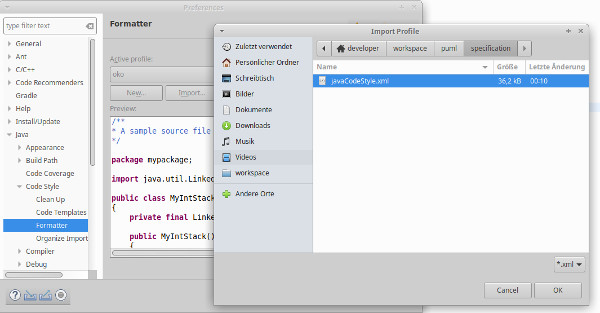
\includegraphics[scale=0.5]{Bilder/importCodeStyle}
\caption{Code-Style in Eclipse importieren}
\end{figure}
Des weiteren empfiehlt es sich bei größeren oder stark geschachtelten Code-Abschnitten die Zugehörigkeit der Schließenden Klammer mit einem Kommentar zu Kennzeichnen.\\
Sonstige Konventionen:
\begin{itemize}
\item{Variablen und Instanzen beginnen kleingeschrieben}
\item{Klassen und Interfaces beginnen mit Großbuchstaben}
\item{Besteht ein Namen aus mehreren zusammengesetzten Wörtern, beginnen alle weiteren Wörter mit Großbuchstaben (keine Unterstriche in Namen verwenden)}
\item{Aussagekräftige Namen verwenden}
\item{Alle Namen auf Englisch}
\item{Die Kommentare auf Deutsch}
\end{itemize}

\nsecend

\nsecbegin{Zu nutzende Werkzeuge}
\begin{itemize}
\item{Eclipse - Entwicklungsumgebung}
\item{GIT - Dateiversionierung}
\item{Meld - Unterschiede zwischen Dateien anzeigen}
\item{Texmaker - Latex-Editor}
\item{GIMP - Bildbearbeitung für das Editieren von Screenshots}
\end{itemize}
\nsecend



\nsecend %Prozess- und Implementationsvorgaben

\end{shownto} %{-, manualDE}
\begin{shownto}{developer}
\nsecbegin{Was wird wie gemacht?}
\nsecbegin{Eclipse}
\nsecbegin{Projekt in Eclipse importieren}
In den workspace wecheln:\\
cd ~/workspace\\
Projekt Klonen:\\
git clone https://gitlab.imn.htwk-leipzig.de/weicker/puml.git\\
Benutzername und Passwort eingeben.\\
In Eclipse "File->Import->Existing Projects into Workspace"\\
%\begin{figure}[hbtp]
%\centering
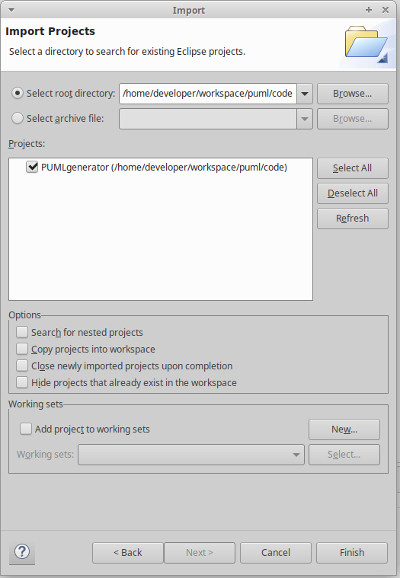
\includegraphics[scale=0.25]{Bilder/importProject}\\
%\caption{Projekt in Eclipse importieren}
%\end{figure}
Dann auf "'Finish"' klicken.
\nsecend

\nsecbegin{WindowBuilder installieren}
In Eclipse "Help->Install New Software..."\\
Unter work with "'2018-09 - http://download.eclipse.org/releases/2018-09"' auswählen.\\
In der Section "'General Purpose Tools"' die im Bild stehenden Häckchen anklicken\\	
\begin{figure}[hbtp]
\centering
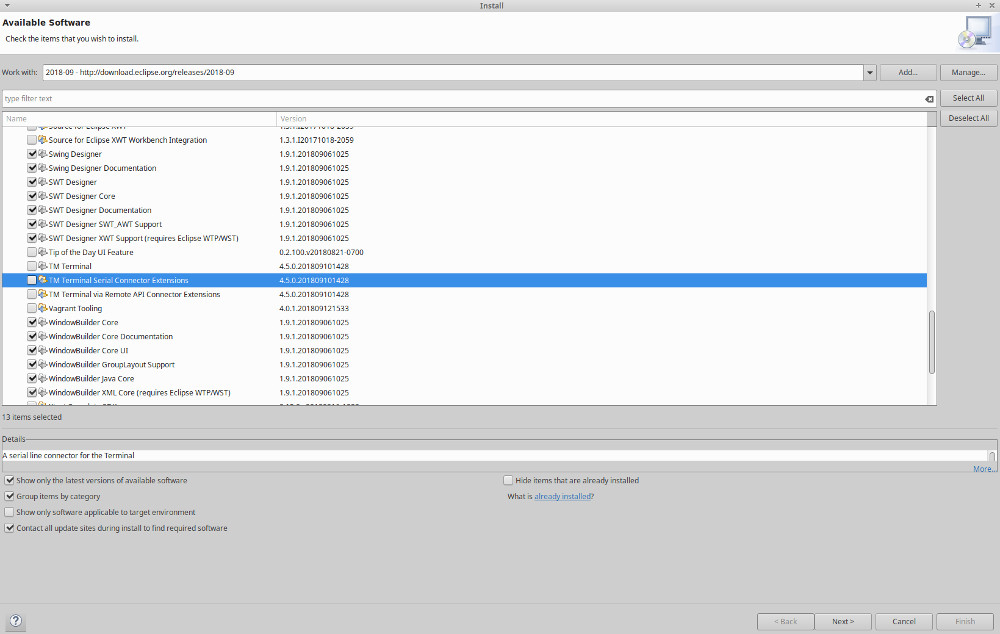
\includegraphics[scale=0.4]{Bilder/installWindowBuilder}\\
\caption{WindowBuilder installieren}
\end{figure}
Dann auf "'Finish"' und sich durch die Installation klicken.
\nsecend

\nsecbegin{GUI editieren}
Es muss der WindowBuilder installiert sein. Dann auf die Datei die die Grafische Oberfläche implementiert (GUI.java) mit der rechten Maustaste klicken. Dann "'Open With->WindowBuilder Editor"' auswählen.
\nsecend
\nsecend %{Eclipse}

\nsecbegin{LaTeX}
\nsecbegin{Geschachtelte Überschriften}
Durch die Makros:
\begin{itemize}
\item \textbackslash nsecbegin\{MeineÜberschrift\}
\item \textbackslash nsecend
\end{itemize}
können geschachtelte Überschriften verwendet werden. Die Kapitel einfach in diese Makros einschließen. Somit muss nicht darauf geachtet werden auf welcher Ebene man sich im Moment befindet. Dies vereinfacht insbesondere das Auslagern von Text in andere Dateien.\\
Um die Makros in die Autovervollständigung des Texmakers aufzunehmen "'Benutzer/in->Wortvervollständigung anpassen"' wählen und dort die Makros hinzufügen.
\begin{figure}[hbtp]
\centering
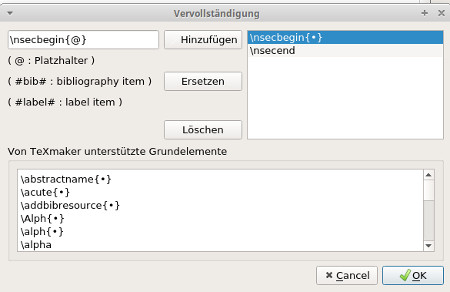
\includegraphics[scale=0.4]{Bilder/autocompleteMakro}
\caption{Autovervollständigung anpassen}
\end{figure}
\nsecend

\nsecbegin{Build-Dateien aufräumen}
Beim erstellen des LaTeX-Dokuments werden jede Menge zusätzliche Dateien erstellt. Dank der entsprechenden "'.gitignore-Datei"' werden diese nicht in GIT hinzugefügt. Für den Fall dass man das Verzeichniss bei sich selbst bereinigen möchte, kann das "'clean.sh"'-Script ausgeführt werden.
\nsecend

\nsecbegin{Entwicklerdokumentation und Handbuch erstellen}
Wenn etwas an der Entwicklerdokumentation oder am Handbuch geändert wurde, müssen diese Dokumente neu erstellt werden. Hierfür zunächst wie gewohnt die LaTeX-Projektdokumentation erstellen. Anschließend kann das "'buildAllDocuments.sh"'-Script ausgeführt werden. Dieses erstellt dann die entsprechenden Dokumente.\\
Weitere Informationen zum "'multiaudience-Paket"' unter \url{https://www.uweziegenhagen.de/?p=3252}.
\nsecend
\nsecend %{Latex}


\nsecbegin{GIT}

\nsecbegin{Benutzername und eMail ins GIT eintragen}
In Linux kann durch den Aufruf:\\
gedit \textasciitilde /.gitconfig\\
die "'.gitconfig-Datei"' editiert werden. In dieser werden unter anderem auch Benutzername und eMail-Addressse des Benutzers gespeichert.
\nsecend

\nsecbegin{Basics}
\begin{lstlisting}[language=bash]
#Aktueller Zustand ausgeben
#Auf Welchem Branch bin ich?
#Gibt es Dateien die geändert sind? 
#Wurden Dateien gelöscht? 
#Wurden neue Dateien hinzugefügt?
#Sind Aenderungen bereits für den Commit vorgemerkt?
#Bin ich vor oder hinter dem Remote-branch?
git status

#Alle Aenderungen für den Commit vormerken.
#Für den Punkt kann auch ein Pfad angegeben werden um bestimmte Änderungen vorzumerken.
#Wenn die .gitignore-Datei richtig gepflegt wird, sollte immer die Variante mit dem Punkt verwendet werden können.
git add .

#Vorgemerkte Änderungen Commiten
#Anschließend muss die Commit-Nachricht im Editor eingetragen werden
git commit

#Alle commits auflisten
git log

#Unterschiede zwischen der aktuellen Version und einem älteren Commit anzeigen
git difftool hashDesCommits

#Unterschiede zwischen zwei aelteren commits anzeigen
git difftool hashDesErstenCommits hashDesZweitenCommits

#Zu einem älteren Commit wechseln
git checkout hashDesCommits

#Neuen Branch vom aktuellen Stand aus erstellen
git branch nameDesNeuenBranches

#Zu einem Branch wechseln
git checkout nameDesBraches

\end{lstlisting}
\nsecend

\nsecbegin{Mergen}
\begin{lstlisting}[language=bash]
#Einen anderen Branch in meinen aktuellen mergen
git merge nameDesBranches

#Bei Merge-Konflikt
git mergetool

#Fuer eine Datei direkt meine Version verwenden 
git checkout --ours -- nameDerKonfliktdatei

#Fuer eine Datei die Remote-version verwenden
git checkout --theirs -- nameDerKonfliktdatei

#Nach dem mergen
git commit
\end{lstlisting}
\nsecend

\nsecbegin{Arbeiten mit dem Server}
\begin{lstlisting}[language=bash]
#Remote anzeigen
git remote -v

#Aktuelle Version eines Branches holen
git pull origin branchName

#Meine Änderungen auf einen Branch hochladen
git push origin branchName
\end{lstlisting}
\nsecend

\nsecbegin{Eigenen Branch mit dem Master Synchronisieren}
Wenn sich der Master wärend der Entwicklung am eigenen Branch weiter entwickelt hat, können die Änderungen des Master auf folgende weise in den eigenen Branch übernommen werden.
\begin{lstlisting}[language=bash]
git status #Pruefen ob auf meinem Branch
#wenn nicht
git checkout myBranch
#Lokalen Master aktuallisieren
git pull origin master #sollte auch gleich in myBranch mergen
#wenn nicht
git merge master
#Wenn merge-konflikt
git mergetool
#Jetzt noch den Merge commiten
git commit
\end{lstlisting}
\nsecend

\nsecbegin{Lokale Branches aufräumen}
ACHTUNG: Sollte nur gemacht werden, wenn alle Änderungen in den Master übernommen wurden und somit sicher sind!!
\begin{lstlisting}[language=bash]
#Alle branches loeschen die es nicht mehr auf dem Server gibt
git remote prune origin
#Lokale branches die mit dem master gemerged wurden loeschen
git branch --merged master | grep -v '^[ *]*master$' | xargs git branch -d
\end{lstlisting}

\nsecend

\nsecend %{GIT}

\nsecbegin{Code}
\nsecbegin{Logger}
%Autor: Patrick Otte
Ein Logger hat verschiedene Level in denen geloggt werden kann:
\begin{itemize}
\item severe	- Schwerwiegende Fehler
\item warning	- Warnungen
\item info	- Informationen
\item config	- Konfigurationshinsweise
\item fine	- Fein
\item finer	- Feiner
\item finest	- Am Feinsten
\end{itemize}
Um nun an einer bestimmten Stelle etwas zu loggen, macht man folgenden Aufruf: \\ \\
PUMLgenerator.logger.getLog().[Level]("[Ausgabe]")\\

Hierbei wird die in der Hauptklasse (PUMLgenerator) definierte Instanz "logger" in Verbindung mit dem Getter getLog() aufgerufen, danach der Level des Logs definiert und am Ende der Ausgabestring eingegeben.\\
Beispiel:\\
PUMLgenerator.logger.getLog().info("Dies ist eine Information");\\
\\
Um die Logs nun auch auf die Konsole auszugeben oder in eine Datei zu schreiben müssen die jeweiligen Handler aktiviert werden. Mit den Funktionen \textit{startLoggingFile(String path)} und \textit{startLoggingConsole(Boolean console)} lassen sich die Handler aktivieren.\\
Beispiel:\\
PUMLgenerator.logger.startLoggingFile("testfolder/tempData/PUMLlog/");\\
\textit{Aktiviert das Schreiben einer Logdatei}\\
PUMLgenerator.logger.startLoggingFile(true);\\
\textit{Aktiviert das Ausgeben auf die Konsole}\\\\


Zum Start des FileHandlers wird eine Logdatei mit exakter Uhrzeit/Datum als Präfix erstellt.
Jeder Logeintrag wird im jeweils angegebenen Ordner gespeichert. Zu jedem Logeintrag gibt es das genaue Datum inkl. Uhrzeit sowie die Informationen in welcher Klasse und in welcher Methode es geloggt wurde.
Des Weiteren werden auch Logausgaben mit den gleichen Eigenschaften (Uhrzeit, Klassenname, ...) über die Console realisiert.\\\\
\textbf{LogMX}\\
Die Logdatei wird in einem XML-Format gespeichert. Um dieses komfortabel auslesen zu können, kann man sich mit Hilfe von
\href{https://logmx.com/download}{LogMX}, einem plattformunabhängigem LogViewer, die Logdatei anschauen und Filtern (nach Klassen, Methoden, Uhrzeit, ...). \\
LogMX kann auf diverse Arten implementiert werden.\\\\
\emph{Linux}\\
Für Linux Distributionen gibt es ein entpackbares Archiv, welches nach dem Download entweder direkt als Anwendung gestartet werden kann. Hierzu muss einfach die logmx.sh ausgeführt werden. Beim Start muss als erstes angegeben werden, wo die Datei zu finden ist und danach ob nur eine Logdatei oder mehrere Logdateien in einem Verzeichnis geöffnet werden sollen. Als nächstes muss das Log Format angegeben werden. Das Log Format für alle PUML-Logs ist Java logging. Final muss nun nur noch Java XML format ausgewählt und der Pfad zur Datei eingegeben werden. Danach kann die Datei gelesen werden.\\\\
Um die Dateien direkt über Eclipse zu öffnen muss man einmalig ein paar Einstellungen vornehmen.\\
Unter
\begin{center}
\rightarrow Window\rightarrow Preferences\rightarrow General\rightarrow Content Types
\end{center}
\\kann man in der Liste Text auswählen und ausklappen. Wenn man jetzt XML markiert (kein ausklappen nötig; gemeint ist nicht XML(Illformed)) kann man in untersten Fenster unter Associated Editors über "Add" einen neuen Editor hinzufügen. Dazu wählt man die logmx.sh Datei aus dem entpackten Ordner aus und speichert die Einstellungen. Wenn man nun via Rechtsklick eine Logdatei in Eclipse auswählt kann man unter "Open With" nun logmx auswählen.\\\\
\emph{Windows}
\\
Für Windows gibt es drei Download-Varianten. Man kann zwei .exe-Installer (mit und ohne Java) herunterladen oder ein gepacktes Archiv, welches ebenfalls eine .exe-Datei enthält. Wie in der Linux-Variante kann man auch hier das Programm allein starten oder auch direkt aus Eclipse heraus. Die Schritte sind bei der Implementierung exakt die selben, wie unter \textit{"Linux"} beschrieben, nur das hier nicht die logmx.sh, sondern die LogMX.exe/LogMX-64.exe ausgewählt werden muss (entweder im Archivordner oder im Installationspfad).
Da LogMX einen Java Path benötigt, muss dieser noch in der Datei startup.conf ergänzt werden.
\nsecend %{Logger}
\nsecend %{Code}

\nsecbegin{Profiler}
\nsecbegin{Installation}
Help > Eclipse Marketplace\\
Search: Profiler > Java Mission Control > Install\\
Nach der Installation sollte in der Symbolleiste ein Icon zum Starten des Profilers erscheinen.
\nsecend
\nsecbegin{Verwendung}
Nach dem Starten wird in dem auftauchenden Fenster unter Local  'Eclipse' und anschließend 'Start JMX Console' ausgewählt.\\
\begin{itemize}
\item Overview\\
Hier sind allgemeine Informationen über die Systembelastungen zu finden.
\item MBean Browser (Managed Beans)\\
MBeans sind Java Objekte, die verwaltet werden können. Das können Geräte, Anwendungen oder andere Ressourcen, die verwaltet werden, sein.\\ Diese können unter diesem Reiter abgerufen werden.
\item Triggers\\
Um verschiedene Events zu testen, können Trigger gesetzt werden. Mittels 'Add' ruft man eine Liste der möglichen Trigger auf und kann diese nach dem Hinzufügen über die Reiter 'Conditions', 'Actions' und Constraints modifizieren.\\
Außerdem lassen sich Trigger importieren sowie exportieren.
\item System\\
Eingie Systeminformationen werden hier angezeigt.
\item Memory\\
Dieser Punkt gibt einen Überblick über Heap und Garbage Collection.
\item Threads\\
Hier findet man eine Liste der laufenden Threads.
\item Diagnostic Commands\\
Die hier aufgelisteten Befehle können hilfreich sein, um spezielle Diagnosen zu erfragen.\\
Dafür wird der entsprechende Befehl ausgewählt, falls nötig unter 'Description - Value' mit Werten versehen und dann kann er ausgeführt werden.
\end{itemize}
Allgemein können die einzelnen Felder durch die '+'-Symbole weiter angepasst werden.
\nsecend
\nsecend %{Profiler}

\nsecbegin{Generell}
\nsecbegin{Graphviz}
%Autor: Patrick Otte
Um PlantUML richtig und im vollem Umfang anzeigen zu können muss Graphviz installiert werden:
\begin{itemize}
\item[1.] Download unter graphviz.org/download/ für jeweiliges System
\item[2.] Folgt den Installationsanweisungen
\item[3.] Graphviz sollte nun erfollgreich installiert sein.
\end{itemize}\\
Graphviz soll für den Endkunden in den Installer implementiert werden.
\nsecend %{Graphviz}
\nsecend %{Generell}

\nsecbegin{XML / XPath}
\nsecbegin{XPath-Ausdrücke ausführen}
Für das Verarbeiten von XPath-Ausdrücken wurde die Methode "'getList"' in der Klasse "'XmlHelperMethods"' erstellt. Von dieser Klasse existiert eine Instanz in der Klasse "'PUMLGenerator"' mit dem Namen "'xmlHelper"'. Ein XPath-Ausdruck kann also folgendermaßen ausgeführt werden:
\begin{lstlisting}
NodeList myNodeList = PUMLGenerator.xmlHelper.getList(myNode, "myXPathExpression");
\end{lstlisting}
Wobei eine List mit allen gefunden Knoten zurückgeliefert wird. Es kann relativ zum übergebenen Knoten (myNode) gesucht werden.
Weitere Informationen zu XPath-Ausdrücken unter:\\
\url{https://www.w3schools.com/xml/xpath_syntax.asp}
\nsecend

\nsecbegin{Nächsten Nachbarknoten suchen}
Weil sich die "'nextSibling"'-Methode der Java-XML-Implementierung etwas seltsam verhält und ggf. die Leerzeichen der Zwischenräume zwischen den Knoten als #text-Knoten erkennt, sollte auch hier ein XPath-Ausdruck verwendet werden. (\url{https://stackoverflow.com/questions/17641496/how-can-i-get-the-siblings-of-an-xml-element-in-java-using-the-dom-parser}) Der Ausdruck:
\begin{lstlisting}
Node nextNode = PUMLGenerator.xmlHelper.getList(currentNode, "following-sibling::*").item(0);
\end{lstlisting}
wählt den nächsten Nachbarknoten aus. Das selbe gilt für die Auswahl des ersten Kindknotens. Der hierfür benötigte Ausdruck:
\begin{lstlisting}
Node childNode = PUMLgenerator.xmlHelper.getList(methodefNode, "child::*").item(0);
\end{lstlisting}
\nsecend
\nsecend %{XML / XPath}

\nsecend %{Was wird wie gemacht?}
\nsecbegin{Best practice}
\nsecbegin{GIT}
\nsecbegin{Keine nicht benötigten Dateien adden}
Vor dem "'git add ."' immer mit "'git status"' prüfen welche Dateien hinzugefügt werden. Sollten nicht für das Projekt benötigte Dateien (z.B. übersetzte Binärdateien oder Dokumentation von Librarys) dabei sein, bitte die entsprechende "'.gitignore-Datei"' vervollständigen. Danach sollten die Dateien beim "'git status"' nicht mehr angezeigt und somit nicht mehr geadded werden.\\
HINWEIS: Die "'.gitignore-Datei"' ist (wie an dem führenden Punkt zu sehen ist) versteckt und wird nur nach dem setzen des entsprechenden Häckchens im Dateimanager oder beim "'ls -a"' angezeigt.
\nsecend
\nsecbegin{Branches nach aktuell zu bearbeitendem Thema benennen}
Damit direkt aus dem Branchname ersichtbar ist was innerhalb des Branches bearbeitet wird, ist es sinnvoll den Name entsprechend zu wählen (Z.B. GUIBranch). Da die Branches mit dem Gitlab-Server synchronisiert werden können, ist es auch ohne weiteres möglich dass mehrere Personen an einem Branch arbeiten.
\nsecend
\nsecend
\nsecend
\end{shownto}

\begin{shownto}{-, developer, manualDE}

%%%%%%%%%%%%
%% Abschnitt mit den Sprints beginnt hier
%%%%%%%%%%%%

\nsecbegin{Sprint 1}

\nsecbegin{Ziel des Sprints}
Es soll eine funktionsfähige Basisversion, welche für das einfache erstellen von Klassendiagrammen aus Java-Code verwendet werden soll entstehen. Das Programm soll sowohl über die Kommandozeile, als auch über eine grafische Oberfläche bedient werden können. Die erzeugten Klassendiagramme sollen in der grafischen Oberfläche angezeigt werden können.

\begin{figure}[hbtp]
\centering
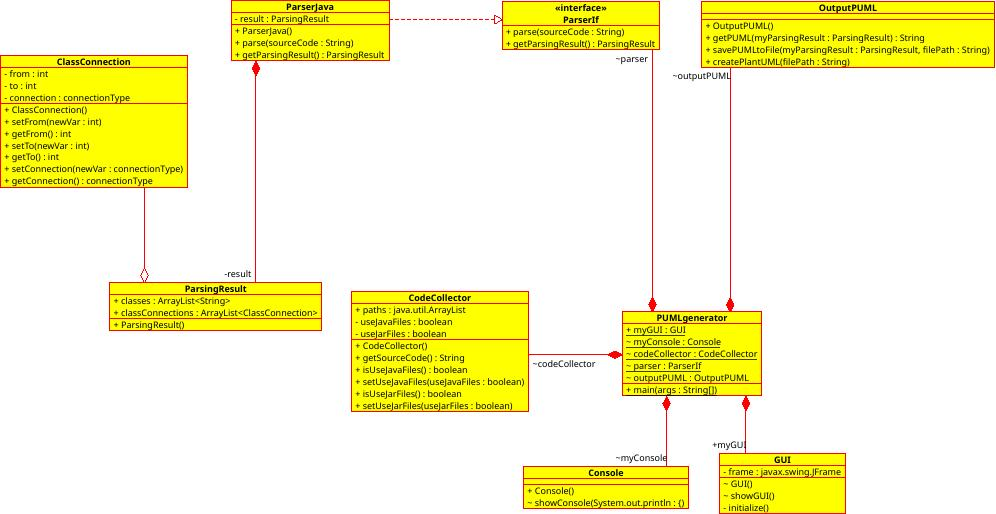
\includegraphics[scale=0.5]{Bilder/classDiagrammSprint1}
\caption{Klassendiagramm des Sprints}
\end{figure}
\nsecend

\nsecbegin{User-Stories des Sprint-Backlogs}
\nsecbegin{Dateien einlesen}
\nsecbegin{Art der eingelesenen Datei}
Als Benutzer wünsche ich mir, dass eine Auswahl zwischen Jar- und Java-Dateien möglich ist, damit Quellcode nicht doppelt eingelesen wird.
\nsecend

\nsecbegin{Java-Dateien}
Als Benutzer wünsche ich mir, dass Java-Dateien einlesbar sind, um den Quellcode von einer oder mehreren Klassen zu analysieren.
\nsecend

\nsecbegin{Jar-Dateien}
Als Benutzer wünsche ich mir, dass Jar-Dateien einlesbar sind, um den Quellcode zu analysieren.
\nsecend
\nsecend

\nsecbegin{Vorschau}
Als Benutzer wünsche ich mir eine Vorschau der Diagramme, damit ich einschätzen kann ob ich damit zufrieden bin.
\nsecend

\nsecbegin{Kommandozeile}
Als Benutzer wünsche ich mir, dass das Programm von der Kommandozeile aus aufrufbar ist, um es automatisiert starten zu können.
\nsecend

\nsecbegin{Klassendiagramme}
Als Benutzer wünsche ich mir, Klassendiagramme aus meinem bestehenden Quellcode erstellen zu können, damit ich das nicht manuell tun muss.
\nsecend

\nsecbegin{Anzeigen und Speichern von PlantUML}
Als Benutzer wünsche ich mir, Diagramme als PlantUML-Code anzeigen und speichern zu können, um den Aufbau nachvollziehen zu können.
\nsecend

\nsecbegin{Plattformunabhängigkeit}
Als Project Owner wünsche ich mir, dass das Programm plattformunabhängig ist, damit es sich gut verbreiten lässt.
\nsecend

\nsecend

\nsecbegin{Liste der durchgeführten Meetings}
\begin{itemize}
\item Planning-Meeting
\end{itemize}
\nsecend

\nsecbegin{Ergebnisse des Planning-Meetings}
Dem gesammten Team ist die geplante Grundstruktur des Programms bekannt. Jeder weis welchen Teil des Programms er implementieren soll.
\nsecend

\nsecbegin{Aufgewendete Arbeitszeit pro Person$+$Arbeitspaket}
\begin{longtable}{|p{4cm}|l|l|l|l|l|}
        \hline
        Arbeitspaket & Person & Start & Ende & h & Artefakt\\
        \hline
        Dummyklassen & Musterstudi & 3.5.09 & 12.5.09 & 14 & Klasse.java\\ \hline
        AP XYZ &  &  &  & & \\ \hline
\end{longtable}     
\nsecend

\nsecbegin{Konkrete Code-Qualität im Sprint}
XXX
\nsecend

\nsecbegin{Konkrete Test-Überdeckung im Sprint}
XXX
\nsecend

\nsecbegin{Ergebnisse des Reviews}
XXX
\nsecend

\nsecbegin{Ergebnisse der Retrospektive}
XXX
\nsecend

\nsecbegin{Abschließende Einschätzung des Product-Owners}
XXX
\nsecend

\nsecbegin{Abschließende Einschätzung des Software-Architekten}
XXX
\nsecend

\nsecbegin{Abschließende Einschätzung des Team-Managers}
XXX
\nsecend


\nsecend

\nsecbegin{Sprint 2}
%% %Autoren: Julian Uebe, Jan Sollmann
\nsecbegin{Ziel des Sprints}
Dieser Sprint ist ausschließlich dazu gedacht, im Verlauf des ersten Sprints identifizierte und noch nicht behobene Bugs zu entfernen. Es wurden bewusst keine neuen User-Stories (für den Benutzer) im Sprint-Backlog definiert. Der Fokus liegt darauf, die im ersten Sprint geschaffene Basis noch einmal zu stabilisieren.
\nsecend

\nsecbegin{User-Stories des Sprint-Backlogs}
\nsecbegin{Reduzierung von Bugs}
Als Softwarearchitekt und Product Owner wünschen wir uns, dass möglichst wenige Bugs auftreten, um die spätere Weiterentwicklung und damit die uneingeschränkte Funktionalität des Produkts nicht zu gefährden.
\nsecend
\nsecend % {User-Stories des Sprint-Backlogs}

\nsecbegin{Zeitliche Planung}
\begin{figure}[hbtp]
\centering
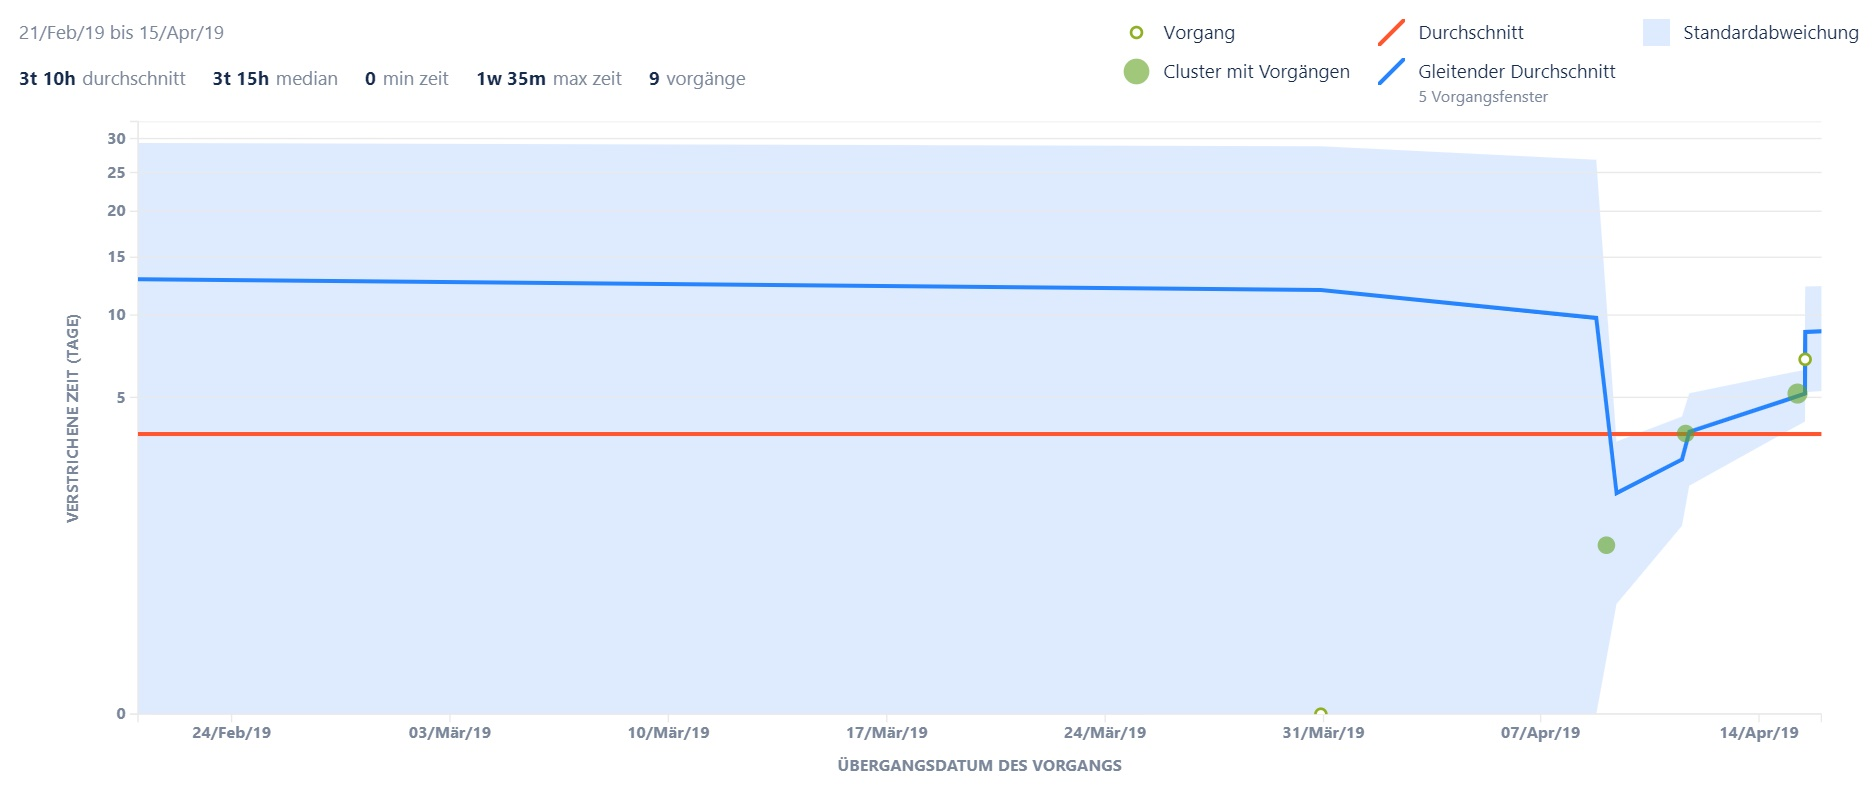
\includegraphics[width=\textwidth]{Bilder/diagram_sprint2}
\caption{Kontroll-Diagramm für Sprint 2}
\end{figure}
\nsecend%Zeitliche Planung

\nsecbegin{Liste der durchgeführten Meetings}
\begin{itemize}
\item Planning-Meeting (21.02.2019)
\item Zwischen-Meeting (08.04.2019)
\item Zwischen-Meeting (11.04.2019)
\item Review-Meeting (15.04.2019)
\end{itemize}
\nsecend%Liste der durchgeführten Meetings

\nsecbegin{Ergebnisse des Planning-Meetings}
Der zweite Sprint wird zeitlich in der letzten Woche der Semesterferien begonnen und bis zum Ende der ersten Woche der Vorlesungszeit gehen. Dies wurde mit den Teammitgliedern besprochen. Hauptziel des Sprints ist ein sauberer Stand, mit dem ab dem kommenden Sommersemester weitergearbeitet werden kann.
\nsecend

\nsecbegin{Aufgewendete Arbeitszeit pro Person$+$Arbeitspaket}
\begin{longtable}{|p{4cm}|l|l|l|l|l|}
        \hline
        Arbeitspaket & Person & Start & Ende & h & Artefakt\\
        \hline
        Testdaten & Marian Geissler   & 06.04.2019 & 15.04.2019 & 2 &  \\ \hline
        Logger & Patrick Otte   & 08.02.2019 & 08.04.2019 & 12 & LogMain.java \\ \hline
        Output & Patrick Otte   & 11.04.2019 & 15.04.2019 & 3 & OutputPUML.java \\ \hline
        Konsole & Johann Gerhardt   & 14.04.2019 & 14.04.2019 & 1 & Console.java \\ \hline
        Java-Parser & Michael Lux   & 30.03.2019 & 30.03.2019 & 14 & ParserJava.java\\ \hline
        GUI & Jan Sollmann  & 01.04.2019 & 06.04.2019 & 5 & GUI\_SWT.java \\ \hline
        GUI & Julian Uebe  & 21.02.2019 & 15.04.2019 & 7 & SWT-Tool \\ \hline
        Code-Collector & Elisabeth Schuster  & 07.02.2019 & 14.04.2019 & 5.5  & CodeCollector.java \\ \hline
        Profiler & Elisabeth Schuster  & 10.04.2019 & 26.04.2019 & 7  & Profiler \\ \hline
       Java-Parser & Jona Meyer  & 30.03.2019 & 30.03.2019 & 7 & ParserJave.java \\ \hline
        Code-Collector & Leo Rauschke  & 07.04.2019 & 14.04.2019 & 5.75 & CodeCollector.java \\ \hline
        Profiler & Leo Rauschke  & 09.04.2019 & 29.04.2019 & 3 & Profiler\\ \hline
        Output & Tore Arndt  & 11.04.2019 & 15.04.2019 & 5 & OutputPUML.java\\ \hline
        
        
\end{longtable}     
\nsecend

\nsecbegin{Konkrete Code-Qualität im Sprint}
Die Codequalität ist etwas besser geworden. Wobei hin und wieder durchaus noch massive Unschönheiten bemängelt werde müssen.
\nsecend

\nsecbegin{Konkrete Test-Überdeckung im Sprint}
Die Testüberdeckung ist auf 40,6\% gesunken.
\nsecend

\nsecbegin{Ergebnisse des Reviews}
\begin{table}[H]

\begin{tabularx}{\textwidth}{ |l|l|X| }
\hline
\textbf{Klasse} & \textbf{Methode} & \textbf{Anmerkungen}\\
 \hline
 
 Testdatensatz & komplett & zukünftig als automatischer Ausgabe-Test\\ \hline
 GUI\_SWT.java & komplett & wird durch Swing-GUI ersetzt\\ \hline
 CodeCollector & Pfadbehandlung & Funktioniert nun auch unter Windows\\ \hline
 CodeCollector & einlesen & Funktioniert\\ \hline
 ParserJava.java & buildTree & Es bestehen weitherhin Bugs\\ \hline
 Alle & komplett & Unit-Tests für das ganze Programm folgen\\ \hline
 ParserJava.java & buildTree & Erweiterung für das Erstellen von Sequenzdiagrammen\\ \hline
 GUI\_SWT.java & createContents, runPUML & Ausgabe für Sequenzdiagramme muss implementiert werden\\ \hline
 
%Console & showConsole & Pfad anpassen \\
\hline
\end{tabularx}
\end{table}

\nsecend%Ergebnisse des Reviews

\nsecbegin{Ergebnisse der Retrospektive}
Die Retrospektive schloss mit einer positiven Bilanz. (...)
\nsecend%Ergebnisse der Retrospektive

\nsecbegin{Abschließende Einschätzung des Product-Owners}
In diesem Sprint wurden einige kritische Bugs behoben und somit User Stories des letzten Sprint-Backlogs noch vervollständigt. Zu hoffen bleibt trotzdem, dass in allen folgenden Sprints auch neue Funktionalität hinzugefügt wird.
\nsecend%Abschließende Einschätzung des Product-Owners

\nsecbegin{Abschließende Einschätzung des Software-Architekten}
Der erste Meilenstein wird als erreicht angesehen, auch wenn der Parser durchaus noch Mängel enthält. Der Grundentwurf der Architektur ist vollständig umgesetzt. Da im nächsten Sprint die Sequenz-Diagramme hinzugenommen sollen, wird hier ein kleiner Umbau der Architektur notwendig sein. Die Klassen ParsingResult, welche nur Daten (unter anderem vom Typ ClassConnection) enthält wird durch XML ersetzt. Dies war von Anfang an vorgesehen, wurde aber aufgrund der höheren Komplexität bisher vermieden. Des weiteren haben wir beschlossen die Sprintdauer auf 2 Wochen zu verkürzen, um die Entwicklung zu beschleunigen.
\nsecend%Abschließende Einschätzung des Software-Architekten

\nsecbegin{Abschließende Einschätzung des Team-Managers}
Insgesamt kann positiv herausgehoben werden, dass sich die Teammitglieder geschlossen dazu bereit erklärten, Teil ihrer Semesterferien für den zweiten Sprint zu opfern. Die Motivation, das Produkt weiter voranzubringen, scheint derzeit ungebrochen.
\nsecend%Abschließende Einschätzung des Team-Managers
\nsecend

%%%%%% weitere Sprints analog


\nsecbegin{Dokumentation}

\nsecbegin{Handbuch}
\end{shownto} %{-, developer, manualDE}
\begin{shownto}{-, developer}
Hier soll das Deutsche Benutzerhandbuch entstehen.
\end{shownto} %{-, developer}
\begin{shownto}{-, developer, manualDE}
\nsecend

\nsecbegin{Installationsanleitung}
XXX
\nsecend

\nsecbegin{Software-Lizenz}
XXX
\nsecend

\nsecend %Dokumentation


\nsecbegin{Projektabschluss}

\nsecbegin{Protokoll der Abnahme und Inbetriebnahme beim Kunden}
XXX
\nsecend

\nsecbegin{Präsentation auf der Messe}
Poster, Bericht
\nsecend

\nsecbegin{Abschließende Einschätzung durch Product-Owner}
XXX
\nsecend

\nsecbegin{Abschließende Einschätzung durch Software-Architekt}
XXX
\nsecend

\nsecbegin{Abschließende Einschätzung durch Team-Manager}
XXX
\nsecend


\nsecend %Projektabschluss

\end{shownto} %{-, developer, manualDE}

\end{document}
